\chapter{Current--Potential Curves}\label{ch:b2:current-potential-curves}

Zinc is electroplated onto steel from acidic baths. Yet the E--pH diagram of
the Year 1 volume says that zinc, far below the hydrogen line, should reduce
the acid and dissolve as fast as it is deposited. It does not, because a
diagram says what may happen, not how fast. The rate of an electrode reaction
is a current, and plotting that current against the electrode potential
shows at once which reactions are fast, which are slow, and which are held
back by the supply of reactant. These \omterm{def:b2:current-potential-curves:ie-curve}{current--potential curves} are the tool
of every electrochemist who plates a metal, charges a battery or measures
oxygen in a river.

\begin{recall}
The Year 1 volume: electrode potential, reference electrode, the Nernst
equation, E--pH diagrams and their limit (they tell what is possible, not how
fast). \Cref{ch:b2:cell-thermodynamics}: $\Delta_r G = -nFE$, the Nernst
equation derived. From physics: diffusion and Fick's law, $j = -D\,dc/dx$.
\end{recall}

\begin{omfigure}
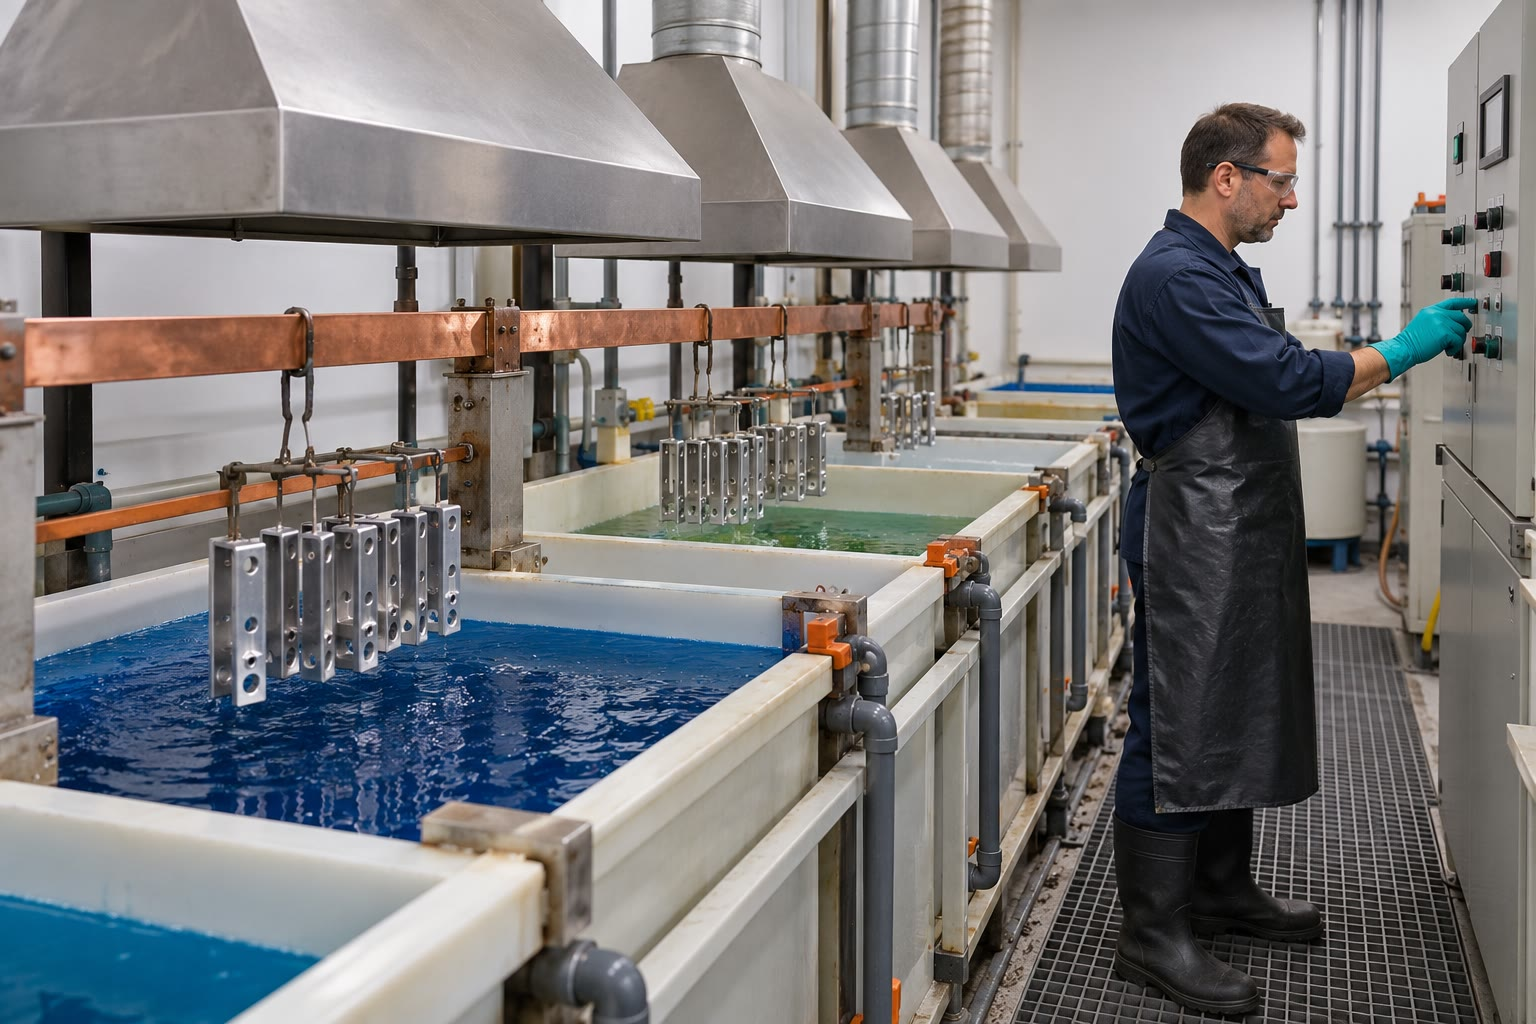
\includegraphics[width=0.62\linewidth]{images/book3/ai/b2-10-electroplating.jpg}

{\small An electroplating line: the parts to be coated hang from copper bus
bars into the baths and are made the cathode; the operator sets the current
at the rectifier. The current fixes how fast metal is deposited; the potential
of the parts decides which metal, or how much hydrogen, is formed with it.}
\end{omfigure}

\section{An electrode out of equilibrium}

\begin{definition}[Current--potential curve]\label{def:b2:current-potential-curves:ie-curve}
The \emph{current--potential curve}\index{current--potential curve} of an
electrode in a solution is the graph of the current $i$ through the electrode
against its potential $E$. An \emph{anodic current}\index{anodic current},
counted positive, corresponds to an oxidation at the electrode; a
\emph{cathodic current}\index{cathodic current}, counted negative, to a
reduction.
\end{definition}

\begin{definition}[Electroactive species]\label{def:b2:current-potential-curves:electroactive}
An \emph{electroactive species}\index{electroactive species} is a species
that can be oxidised or reduced at the electrode in the range of potentials
considered.
\end{definition}

\begin{proposition}[Current and rate]\label{prop:b2:current-potential-curves:current-rate}
If a single half-reaction with $n$ electrons takes place at an electrode, the
current measures its rate: $i = nF\,d\xi/dt$, with $\xi$ the advancement of
the oxidation (so that $i > 0$ for an oxidation, $i < 0$ for a reduction).
\end{proposition}

\begin{proof}
By \cref{prop:b2:cell-thermodynamics:charge}, an advancement $d\xi$ moves the
charge $nF\,d\xi$ through the electrode in time $dt$.
\end{proof}

To record such a curve, the potential of one electrode must be imposed and
measured while a current flows through it --- which a two-electrode cell
cannot do, since the current also changes the potential of the second
electrode.

\begin{definition}[Three-electrode set-up]\label{def:b2:current-potential-curves:set-up}
In a three-electrode set-up, the current flows between the \emph{working
electrode}\index{working electrode}, the one studied, and the \emph{counter
electrode}\index{counter electrode}, which closes the circuit; the potential
of the working electrode is measured against a reference electrode through
which no current flows. An electronic potentiostat adjusts the current so
that this potential keeps the imposed value.
\end{definition}

\begin{omfigure}
\begin{tikzpicture}[font=\small, >={Stealth}]
  \pic[transform shape] at (0,0) {beaker={0.7}{omDef!14}};
  \pic at (-0.55,0.25) {electrode={black!35}};
  \pic at (0.55,0.25) {electrode={black!15}};
  \pic (r) at (0.0,0.15) {probe};
  \draw[thick, rounded corners] (-2.2,4.3) rectangle (2.2,5.5);
  \node at (0,4.9) {potentiostat};
  \draw[thick, omThm] (-0.40,2.65) -- (-0.40,3.5) -- (-1.6,3.5) -- (-1.6,4.3);
  \draw[thick, omDef] (0.70,2.65) -- (0.70,3.5) -- (1.6,3.5) -- (1.6,4.3);
  \draw[thick] (r-top) -- (0,4.3);
  \node[anchor=east, font=\scriptsize, omThm] at (-1.65,3.85) {WE};
  \node[anchor=west, font=\scriptsize, omDef] at (1.65,3.85) {CE};
  \node[anchor=west, font=\scriptsize] at (0.05,3.95) {RE};
  \draw[<-, omProp, thick] (-0.75,1.2) -- (-2.0,1.4) node[left, text=black, align=right] {working\\ electrode};
  \draw[<-, omProp, thick] (0.85,1.2) -- (2.1,1.4) node[right, text=black, align=left] {counter\\ electrode};
  \draw[<-, omProp, thick] (0.05,0.5) -- (1.4,-0.4) node[right, text=black] {reference electrode};
  \node[font=\scriptsize, align=center] at (0,6.0) {imposes $E_{\text{WE}} - E_{\text{RE}}$, measures $i$};
\end{tikzpicture}

{\small The three-electrode set-up. The potentiostat drives the current
between the \omterm{def:b2:current-potential-curves:set-up}{working electrode} (WE) and the \omterm{def:b2:current-potential-curves:set-up}{counter electrode} (CE) so as to
hold the potential of the \omterm{def:b2:current-potential-curves:set-up}{working electrode}, measured against the reference
electrode (RE), at the imposed value; no current flows through the
reference.}
\end{omfigure}

When no current flows and both forms of a couple are present, the electrode
takes the Nernst potential of the couple --- if the electron exchange is fast
enough to establish it. Moving the potential away from it makes a current
flow.

\section{Fast and slow systems}

\begin{definition}[Overpotential]\label{def:b2:current-potential-curves:overpotential}
The \emph{overpotential}\index{overpotential} of an electrode through which a
current $i$ flows is $\eta = E(i) - E_{\text{eq}}$, the difference between its
potential and the equilibrium (Nernst) potential of the couple. The
\emph{threshold potential}\index{threshold potential} of a half-reaction is the
potential beyond which its current becomes noticeable.
\end{definition}

\begin{definition}[Fast and slow systems]\label{def:b2:current-potential-curves:fast-slow}
A couple is a \emph{fast system}\index{fast system} at a given electrode if a
noticeable current flows as soon as the potential departs from its Nernst
potential; it is a \emph{slow system}\index{slow system} if an \omterm{def:b2:current-potential-curves:overpotential}{overpotential} of
some tenths of a volt is needed before the current becomes noticeable, in
either direction.
\end{definition}

Whether a system is fast or slow depends on the couple and on the electrode
material. The \ce{Fe^3+}/\ce{Fe^2+} and \ce{Ag+}/\ce{Ag} couples are fast on
platinum; the reduction of \ce{H+} is fast on platinum but slow on mercury,
lead or zinc; the oxidation of water to dioxygen is slow on every electrode.
Electron transfers that break or form bonds, like those of \ce{O2} or \ce{H2},
are typically slow; the transfer of an electron between two ions of nearly the
same shape is fast. The shape of the rising part of a slow curve comes from
the kinetics of electron transfer, derived in the Year 3 volume.

\begin{omfigure}
\begin{tikzpicture}
\begin{axis}[omie, width=0.47\linewidth, height=5.4cm, xmin=0.25, xmax=1.3,
  ymin=-1.3, ymax=1.3, xlabel={$E$}, ylabel={$i$}, title={\small fast system}]
\addplot[omanodic] table[x=E, y=i, restrict expr to domain={\thisrow{i}}{0:2}] {figdata/out/bachelor-2-ie-curves-a.dat};
\addplot[omcathodic] table[x=E, y=i, restrict expr to domain={\thisrow{i}}{-2:0}] {figdata/out/bachelor-2-ie-curves-a.dat};
\draw[densely dotted] (axis cs:0.77,-1.2) -- (axis cs:0.77,1.2);
\node[font=\scriptsize, anchor=north west] at (axis cs:0.78,-0.05) {$E_{\text{eq}}$};
\node[font=\scriptsize, anchor=south] at (axis cs:1.1,1.0) {\ce{Fe^2+} $\to$ \ce{Fe^3+}};
\node[font=\scriptsize, anchor=north] at (axis cs:0.45,-1.0) {\ce{Fe^3+} $\to$ \ce{Fe^2+}};
\end{axis}
\end{tikzpicture}\hfill
\begin{tikzpicture}
\begin{axis}[omie, width=0.47\linewidth, height=5.4cm, xmin=-0.25, xmax=1.8,
  ymin=-1.3, ymax=1.3, xlabel={$E$}, ylabel={$i$}, title={\small slow system}]
\addplot[omanodic] table[x=E, y=i, restrict expr to domain={\thisrow{i}}{0:2}] {figdata/out/bachelor-2-ie-curves-c.dat};
\addplot[omcathodic] table[x=E, y=i, restrict expr to domain={\thisrow{i}}{-2:0}] {figdata/out/bachelor-2-ie-curves-c.dat};
\draw[densely dotted] (axis cs:0.77,-1.2) -- (axis cs:0.77,1.2);
\draw[<->, omProp] (axis cs:0.77,0.5) -- (axis cs:1.12,0.5) node[midway, above, font=\scriptsize] {$\eta_a$};
\draw[<->, omProp] (axis cs:0.42,-0.5) -- (axis cs:0.77,-0.5) node[midway, below, font=\scriptsize] {$\eta_c$};
\node[font=\scriptsize, anchor=north west] at (axis cs:0.78,-0.05) {$E_{\text{eq}}$};
\end{axis}
\end{tikzpicture}

{\small Model \omterm{def:b2:current-potential-curves:ie-curve}{current--potential curves} of a couple whose two forms are present
at equal concentrations (anodic branch red, cathodic blue). Left, a \omterm{def:b2:current-potential-curves:fast-slow}{fast
system}: the current changes sign steeply at the equilibrium potential. Right,
a \omterm{def:b2:current-potential-curves:fast-slow}{slow system}: no current flows over a range of potentials around it; each
branch needs an \omterm{def:b2:current-potential-curves:overpotential}{overpotential}. Both reach the same limiting plateaus, set by
diffusion. (Illustrative values.)}
\end{omfigure}

\section{Mass transport and limiting currents}

When the electron transfer is fast, the current is limited by the arrival of
the reactant at the electrode. In a stirred solution, a thin layer of liquid
next to the electrode stays nearly still, and the reactant crosses it by
diffusion.

\begin{definition}[Diffusion layer and limiting current]\label{def:b2:current-potential-curves:limiting-current}
The \emph{diffusion layer}\index{diffusion layer} is the layer of solution,
of thickness $\delta$ (a few to some tens of micrometres in a stirred
solution), next to the electrode, across which species move by diffusion
only. The \emph{limiting current}\index{limiting current} is the current
reached when the \omterm{def:b2:current-potential-curves:electroactive}{electroactive species} is consumed as fast as it arrives, its
concentration at the surface being zero.
\end{definition}

\begin{omfigure}
\begin{tikzpicture}[font=\small, >={Stealth}, x=1.2cm, y=1.2cm]
  \fill[black!25] (-0.4,0) rectangle (0,3);
  \node[rotate=90, font=\scriptsize] at (-0.2,1.5) {electrode};
  \draw[->] (0,0) -- (4.6,0) node[right] {$x$};
  \draw[->] (0,0) -- (0,3.2) node[above] {$c$};
  \draw[densely dashed] (1.6,0) -- (1.6,3);
  \node[below, font=\scriptsize] at (1.6,0) {$\delta$};
  \draw[omDef, thick] (0,1.2) -- (1.6,2.4) -- (4.4,2.4);
  \draw[omThm, thick] (0,0.02) -- (1.6,2.4);
  \node[font=\scriptsize, anchor=west] at (2.6,2.6) {bulk, $c^b$ (stirred)};
  \node[font=\scriptsize, omDef, anchor=east] at (-0.45,1.2) {$c^s$};
  \node[font=\scriptsize, omThm, anchor=west] at (1.7,0.5) {$c^s = 0$: limiting current};
  \node[font=\scriptsize, align=center] at (0.8,3.0) {diffusion\\ layer};
\end{tikzpicture}

{\small Concentration of the reactant near an electrode in a stirred
solution. Across the \omterm{def:b2:current-potential-curves:limiting-current}{diffusion layer} the profile is linear; the flux, hence the
current, is proportional to $c^b - c^s$. It is largest when the reactant is
consumed as soon as it arrives ($c^s = 0$, red).}
\end{omfigure}

\begin{theorem}[Limiting current]\label{thm:b2:current-potential-curves:limiting}
For a species of bulk concentration $c$ and diffusion coefficient $D$,
crossing a \omterm{def:b2:current-potential-curves:limiting-current}{diffusion layer} of thickness $\delta$ to an electrode of area $A$,
the \omterm{def:b2:current-potential-curves:limiting-current}{limiting current} is, in absolute value,
\[
  |i_{\lim}| = \frac{nFADc}{\delta} .
\]
\end{theorem}

\begin{proof}
At steady state the concentration profile in the layer is linear (Fick's
second law with $\partial c/\partial t = 0$ gives $d^2c/dx^2 = 0$), so the flux
towards the electrode is $j = D(c - c^s)/\delta$, in moles per unit area and
time. Every molecule arriving reacts with $n$ electrons: $|i| = nFAj =
nFAD(c - c^s)/\delta$, largest for $c^s = 0$.
\end{proof}

\begin{example}[Size of a limiting current]\label{ex:b2:current-potential-curves:ilim}
For a species at \qty{10}{mmol/L} (\qty{10}{mol/m^3}), with $D =
\qty{7e-10}{m^2/s}$, $\delta = \qty{20}{\micro m}$, $n = 1$, on
\qty{1.0}{cm^2}: $|i_{\lim}| = 96\,485 \times 10^{-4} \times 7 \times 10^{-10}
\times 10/(2 \times 10^{-5}) = \qty{3.4}{mA}$.
\end{example}

\begin{theorem}[Wave of a fast system]\label{thm:b2:current-potential-curves:wave}
For a fast couple $\mathrm{Ox} + n\,\mathrm e^- \rightleftharpoons \mathrm{Red}$,
with anodic \omterm{def:b2:current-potential-curves:limiting-current}{limiting current} $i_{\lim,a} > 0$ (set by Red) and cathodic
\omterm{def:b2:current-potential-curves:limiting-current}{limiting current} $i_{\lim,c} < 0$ (set by Ox), the steady-state curve is
\[
  E = E_{1/2} + \frac{RT}{nF}\ln\frac{i - i_{\lim,c}}{i_{\lim,a} - i},
  \qquad E_{1/2} = E^\circ + \frac{RT}{nF}\ln\frac{D_{\text{Red}}}{D_{\text{Ox}}} ,
\]
the layer thickness being the same for both forms.
\end{theorem}

\begin{proof}
\omterm{def:b2:current-potential-curves:fast-slow}{Fast system}: the Nernst equation holds at the surface, $E = E^\circ + (RT/nF)
\ln(c^s_{\text{Ox}}/c^s_{\text{Red}})$. Linear profiles: an \omterm{def:b2:current-potential-curves:ie-curve}{anodic current} $i$
consumes Red and produces Ox at the surface, $i = nFAD_{\text{Red}}(c^b_{\text{Red}}
- c^s_{\text{Red}})/\delta = -nFAD_{\text{Ox}}(c^b_{\text{Ox}} - c^s_{\text{Ox}})/\delta$.
With $i_{\lim,a} = nFAD_{\text{Red}}c^b_{\text{Red}}/\delta$ and $i_{\lim,c} =
-nFAD_{\text{Ox}}c^b_{\text{Ox}}/\delta$, these give $c^s_{\text{Red}} = (i_{\lim,a} -
i)\delta/(nFAD_{\text{Red}})$ and $c^s_{\text{Ox}} = (i - i_{\lim,c})\delta/(nFAD_{\text{Ox}})$.
Substitute in the Nernst equation.
\end{proof}

\begin{corollary}[Half-wave potential]\label{cor:b2:current-potential-curves:half-wave}
When the two forms have equal diffusion coefficients, $E_{1/2} = E^\circ$: with
only one form present, the current is half its limiting value at the standard
potential of the couple.
\end{corollary}

\begin{proof}
With only Red present, $i_{\lim,c} = 0$, and for $i = i_{\lim,a}/2$ the logarithm
vanishes: $E = E_{1/2} = E^\circ$ when $D_{\text{Red}} = D_{\text{Ox}}$.
\end{proof}

\begin{proposition}[Plateaus measure concentrations]\label{prop:b2:current-potential-curves:plateau}
At fixed stirring and electrode, the height of a plateau is proportional to the
concentration of the species that it consumes: an electrode held at a
potential on the plateau is an amperometric sensor.
\end{proposition}

\begin{proof}
$|i_{\lim}| = (nFAD/\delta)\,c$ and the factor in brackets is constant at fixed
stirring and temperature.
\end{proof}

\begin{omfigure}
\begin{tikzpicture}
\begin{axis}[omie, width=0.47\linewidth, height=5.0cm, xmin=0.25, xmax=1.3,
  ymin=-0.3, ymax=1.3, xlabel={$E$}, ylabel={$i$}, title={\small only \ce{Fe^2+} present}]
\addplot[omanodic] table[x=E, y=i] {figdata/out/bachelor-2-ie-curves-b.dat};
\draw[densely dotted] (axis cs:0.77,0) -- (axis cs:0.77,0.5) -- (axis cs:0.25,0.5);
\node[font=\scriptsize, anchor=north] at (axis cs:0.77,-0.02) {$E_{1/2}$};
\node[font=\scriptsize, anchor=south west] at (axis cs:0.27,0.5) {$i_{\lim}/2$};
\node[font=\scriptsize, anchor=south] at (axis cs:1.12,1.0) {plateau};
\end{axis}
\end{tikzpicture}\hfill
\begin{tikzpicture}
\begin{axis}[width=0.42\linewidth, height=5.0cm, xmin=0, xmax=1.05, ymin=0, ymax=1.1,
  axis x line=bottom, axis y line=left, xtick=\empty, ytick=\empty,
  xlabel={$c$}, ylabel={$i_{\lim}$}, label style={font=\small},
  title={\small amperometry}]
\addplot[omanodic, mark=*, mark size=1.2pt] table[x=c, y=i] {figdata/out/bachelor-2-ie-curves-e.dat};
\end{axis}
\end{tikzpicture}

{\small Left: the wave of a fast couple when only the reduced form is present
(model); its half-height lies at the half-wave potential. Right: the plateau
height grows in proportion to the concentration.}
\end{omfigure}

\section{The solvent and the electrode}

Water is itself electroactive: it is oxidised to dioxygen
(\ce{2H2O -> O2 + 4H+ + 4e-}) and reduced to dihydrogen (\ce{2H+ + 2e- -> H2}, or
\ce{2H2O + 2e- -> H2 + 2OH-}). As the solvent is never exhausted, its curves
have no plateau: they rise steeply and bound every other curve.

\begin{definition}[Electroactivity window]\label{def:b2:current-potential-curves:window}
The \emph{solvent walls}\index{solvent wall} are the steep branches of the
oxidation and reduction of the solvent. The \emph{electroactivity
window}\index{electroactivity window} is the range of potentials between them,
in which the curves of the dissolved species can be observed.
\end{definition}

\begin{proposition}[The window of water]\label{prop:b2:current-potential-curves:window}
In water at a given pH the window lies around the thermodynamic range of the
two couples of water, $\qty{0}{V} - 0.059\,\mathrm{pH}$ and $\qty{1.23}{V} -
0.059\,\mathrm{pH}$, widened on each side by the \omterm{def:b2:current-potential-curves:overpotential}{overpotential} of the
corresponding reaction on the electrode used.
\end{proposition}

\begin{proof}[Argument]
Each wall starts near the Nernst potential of its couple shifted by the
threshold \omterm{def:b2:current-potential-curves:overpotential}{overpotential}: the oxidation of water is slow on all electrodes, so
the anodic wall lies some tenths of a volt above \qty{1.23}{V} (at pH 0); the
reduction of \ce{H+} is fast on platinum, whose cathodic wall stays close to
\qty{0}{V}, but slow on zinc, lead or mercury, whose wall lies several tenths of
a volt lower.
\end{proof}

\begin{omfigure}
\begin{tikzpicture}
\begin{axis}[omie, width=0.82\linewidth, height=5.4cm, xmin=-1.2, xmax=2.0,
  ymin=-3, ymax=3, xlabel={$E$ (V)}, ylabel={$i$}, clip=true, clip mode=individual]
\addplot[omwall] table[x=E, y=i] {figdata/out/bachelor-2-ie-curves-d-high.dat};
\addplot[omcathodic] table[x=E, y=i, restrict expr to domain={\thisrow{E}}{-1.2:0.6}] {figdata/out/bachelor-2-ie-curves-d-Pt.dat};
\addplot[omanodic] table[x=E, y=i, restrict expr to domain={\thisrow{E}}{0.6:2.0}] {figdata/out/bachelor-2-ie-curves-d-Pt.dat};
\draw[densely dotted] (axis cs:0,-2.8) -- (axis cs:0,2.8);
\draw[densely dotted] (axis cs:1.23,-2.8) -- (axis cs:1.23,2.8);
\node[font=\scriptsize, anchor=north west] at (axis cs:0.02,-0.1) {0};
\node[font=\scriptsize, anchor=north west] at (axis cs:1.24,-0.1) {1.23};
\node[font=\scriptsize, omDef, anchor=west] at (axis cs:0.05,-2.2) {\ce{H+} $\to$ \ce{H2} on Pt};
\node[font=\scriptsize, gray, anchor=east] at (axis cs:-0.85,-1.0) {on Zn, Pb};
\node[font=\scriptsize, omThm, anchor=east] at (axis cs:1.18,2.2) {\ce{H2O} $\to$ \ce{O2}};
\end{axis}
\end{tikzpicture}

{\small The walls of water at pH 0 (model). The reduction of \ce{H+} starts near
\qty{0}{V} on platinum (blue) but several tenths of a volt lower on metals such
as zinc or lead (dashed); the oxidation of water needs an \omterm{def:b2:current-potential-curves:overpotential}{overpotential} on any
electrode. The window is the range between the walls.}
\end{omfigure}

\section{Reading curves}

\begin{method}[Sketching the curves of a solution]\label{met:b2:current-potential-curves:sketch-ie}
\begin{enumerate}
  \item Draw the two walls of the solvent for the pH and the electrode
        material.
  \item For each couple present, place its Nernst potential (both forms
        present) or $E^\circ$ (one form): a \omterm{def:b2:current-potential-curves:fast-slow}{fast system} crosses the axis there
        steeply; a \omterm{def:b2:current-potential-curves:fast-slow}{slow system} is shifted by its \omterm{def:b2:current-potential-curves:overpotential}{overpotentials}.
  \item Give each wave a plateau proportional to the concentration of the
        species it consumes; a metal electrode that oxidises itself has no
        plateau (the metal is not exhausted).
  \item Add the currents of the reactions possible at each potential.
\end{enumerate}
\end{method}

\begin{method}[Reading the curves]\label{met:b2:current-potential-curves:read-ie}
\begin{enumerate}
  \item At an imposed potential, read on each curve the current of each
        reaction: they run simultaneously, in proportion to their currents.
  \item At an imposed current (electrolysis), find the potential at which the
        anodic or cathodic curves add up to that current; the reactions
        involved are those whose curves contribute there.
  \item For a cell, or a corroding metal, the \omterm{def:b2:current-potential-curves:ie-curve}{anodic current} of one reaction
        equals the \omterm{def:b2:current-potential-curves:ie-curve}{cathodic current} of the other: look for that pair of
        points.
\end{enumerate}
\end{method}

\begin{example}[Zinc plating from an acidic bath]\label{ex:b2:current-potential-curves:zinc}
In an acidic zinc bath, the cathode carries two possible reductions: \ce{Zn^2+
+ 2e- -> Zn} ($E^\circ = \qty{-0.76}{V}$, fast) and \ce{2H+ + 2e- -> H2}
($E^\circ = \qty{0}{V}$). Thermodynamically, hydrogen should come first and zinc
never. But on zinc the reduction of \ce{H+} is slow: its wall lies below
\qty{-0.76}{V}, and at the potential where zinc is deposited at a useful
rate, little hydrogen is formed. The curve, not the diagram, explains the
plating.
\end{example}

\begin{history}[Polarography]
\begin{minipage}[t]{0.25\linewidth}
\vspace{0pt}
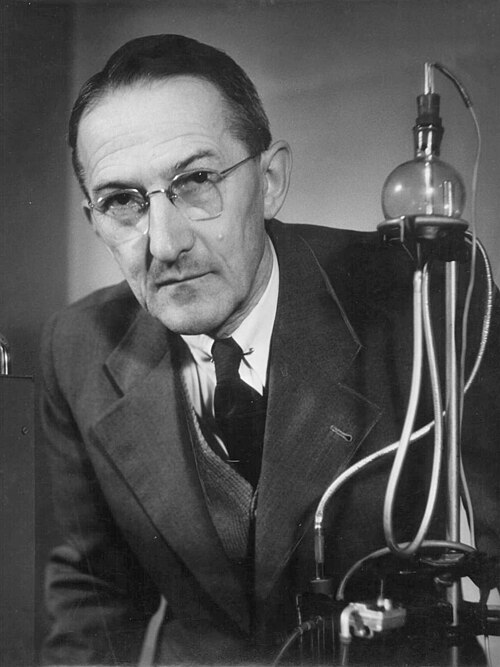
\includegraphics[width=\linewidth]{images/book3/heyrovsky.jpg}
\end{minipage}\hfill
\begin{minipage}[t]{0.71\linewidth}
\vspace{0pt}
In 1922 Jaroslav Heyrovsk\'y recorded the current through a mercury electrode
that formed drop after drop at the tip of a capillary, while the potential was
swept: each reducible species gave a step whose position identified it and
whose height measured its concentration. The renewed drop kept the surface
fresh, and the high \omterm{def:b2:current-potential-curves:overpotential}{overpotential} of hydrogen on mercury opened a wide
cathodic window. Polarography earned him the Nobel Prize in Chemistry in 1959
and founded electroanalytical chemistry; the photograph shows him with a
dropping-mercury electrode. (Photograph: archive of the J.~Heyrovsk\'y
Institute of Physical Chemistry, CC BY-SA 3.0, Wikimedia Commons.)
\end{minipage}
\end{history}

\section{Exercises}

\begin{exercise}[$\star$]\label{exo:b2:current-potential-curves:1}
In a Daniell cell delivering a current, give the sign of the current at the
zinc electrode and at the copper electrode, with the conventions of this
chapter.
\end{exercise}

\begin{exercise}[$\star$]\label{exo:b2:current-potential-curves:2}
Compute the \omterm{def:b2:current-potential-curves:limiting-current}{limiting current} of the reduction of \ce{Ag+} (\qty{2.0}{mmol/L}, $D =
\qty{1.6e-9}{m^2/s}$) on \qty{0.50}{cm^2} with $\delta = \qty{25}{\micro m}$
(model values).
\end{exercise}

\begin{exercise}[$\star$]\label{exo:b2:current-potential-curves:3}
On the model curves of the chapter, how do you recognise a fast and a \omterm{def:b2:current-potential-curves:fast-slow}{slow
system}? Give one example of each on platinum.
\end{exercise}

\begin{exercise}[$\star$]\label{exo:b2:current-potential-curves:4}
A solution contains only \ce{Fe^2+}. At what potential does its \omterm{def:b2:current-potential-curves:ie-curve}{anodic current}
reach half its plateau, if the two forms diffuse alike ($E^\circ = \qty{0.77}{V}$)?
\end{exercise}

\begin{exercise}[$\star\star$]\label{exo:b2:current-potential-curves:5}
A platinum electrode in a solution of \ce{Fe^3+} and \ce{Cu^2+} (equal
concentrations, $E^\circ$ = 0.77 and \qty{0.34}{V}) is swept towards negative
potentials. Describe the curve: waves, plateaus, their heights, and the
cathodic wall.
\end{exercise}

\begin{exercise}[$\star\star$]\label{exo:b2:current-potential-curves:6}
In the solution of \cref{exo:b2:current-potential-curves:5}, the potential of
the electrode is held at \qty{0.50}{V}, then at \qty{0.10}{V}. What happens in
each case?
\end{exercise}

\begin{exercise}[$\star\star$]\label{exo:b2:current-potential-curves:7}
Give the Nernst potentials of the two couples of water at pH 0 and pH 14, and
sketch how the window on platinum moves with pH.
\end{exercise}

\begin{exercise}[$\star\star$]\label{exo:b2:current-potential-curves:8}
\ce{Fe^2+} is titrated by \ce{Ce^4+} while a platinum electrode held at
\qty{1.0}{V} records the current. Sketch the current against the volume added
and explain how it locates the equivalence (\ce{Ce^4+}/\ce{Ce^3+}: $E^\circ =
\qty{1.72}{V}$).
\end{exercise}

\begin{exercise}[$\star\star$]\label{exo:b2:current-potential-curves:9}
Doubling the stirring speed halves the thickness of the \omterm{def:b2:current-potential-curves:limiting-current}{diffusion layer}. What
happens to the plateaus, the half-wave potential and the zero-current
potential of a \omterm{def:b2:current-potential-curves:fast-slow}{fast system}?
\end{exercise}

\begin{exercise}[$\star\star\star$]\label{exo:b2:current-potential-curves:10}
Derive the equation of the wave of a \omterm{def:b2:current-potential-curves:fast-slow}{fast system} with only Red present, and
show that a plot of $E$ against $\log[i/(i_{\lim} - i)]$ is a straight line of
slope $0.059/n$ volt at \qty{25}{\degreeCelsius}.
\end{exercise}

\begin{exercise}[$\star\star\star$]\label{exo:b2:current-potential-curves:11}
A piece of zinc dipped into \qty{1}{mol/L} acid dissolves only slowly, while
the same piece touching a platinum wire dissolves fast, with hydrogen bubbling
on the platinum. Explain with \omterm{def:b2:current-potential-curves:ie-curve}{current--potential curves}.
\end{exercise}

\begin{exercise}[$\star\star\star$]\label{exo:b2:current-potential-curves:12}
To oxidise a species whose wave lies at \qty{2.0}{V} at pH 0, would you choose a
platinum electrode or one with a high oxygen \omterm{def:b2:current-potential-curves:overpotential}{overpotential}? Explain, and say
what would be formed otherwise.
\end{exercise}

\section{Problem: An Oxygen Probe for a River}

\begin{problem}[{Weekend problem --- the cathode of an amperometric oxygen
sensor, the limiting current through its membrane, the calibration in
air-saturated water with Henry's law, and the oxygen content of a river}]
\label{pb:b2:current-potential-curves:1}
An amperometric oxygen probe has a gold cathode and a silver anode in a
potassium chloride gel, separated from the sample by a thin gas-permeable
membrane. The cathode is held at \qty{-0.60}{V} against the silver--silver
chloride anode. Data at \qty{25}{\degreeCelsius}: \omterm{prop:b2:chemical-potential:henry}{Henry's law} constant of
\ce{O2}, $H = \qty{1.3e-5}{mol/(m^3.Pa)}$; vapour pressure of water
\qty{3.17}{kPa}; oxygen in dry air 20.95~\% by volume; $E^\circ(\ce{O2}/\ce{H2O}) =
\qty{1.229}{V}$; $E^\circ(\ce{AgCl}/\ce{Ag}) = \qty{0.222}{V}$. Membrane (model
values): area \qty{0.10}{cm^2}, thickness \qty{25}{\micro m}, effective
diffusion coefficient of \ce{O2} across it \qty{1.0e-10}{m^2/s}.
% ledger: henry:O2, pvap:H2O.298, air:O2, dfg:Cl-_ao, dfg:AgCl_cr, aw:O

\medskip
\noindent\textbf{Part I --- The cathode.}
\begin{enumerate}
  \item Write the reduction of dioxygen in a neutral medium.
  \item Write the reaction at the silver anode, and the overall reaction.
  \item Compute the Nernst potential of the \ce{O2}/\ce{H2O} couple at pH 7 with
        $p_{\ce{O2}} = \qty{0.21}{bar}$.
  \item Express the cathode potential, \qty{-0.60}{V} against Ag/AgCl, on the
        hydrogen scale, taking the chloride activity of the gel as 1.
  \item Why must the cathode be held far below the Nernst potential of
        \ce{O2}?
  \item Why is a potential on the plateau chosen?
  \item What sets the lower limit of the usable potentials?
\end{enumerate}

\medskip
\noindent\textbf{Part II --- The \omterm{def:b2:current-potential-curves:limiting-current}{limiting current}.}
\begin{enumerate}[resume]
  \item Describe the concentration profile of \ce{O2} across the membrane when the
        cathode works on its plateau.
  \item Write the flux of \ce{O2} through the membrane.
  \item Deduce the current as a function of the concentration $c$ of dissolved
        \ce{O2}.
  \item Why is the membrane thickness used in place of the \omterm{def:b2:current-potential-curves:limiting-current}{diffusion layer}?
  \item Why does the reading depend little on the stirring of the river, but a
        lot on fouling of the membrane?
\end{enumerate}

\medskip
\noindent\textbf{Part III --- Calibration.}
\begin{enumerate}[resume]
  \item Compute the partial pressure of \ce{O2} over water saturated with air at
        \qty{1.013}{bar} and \qty{25}{\degreeCelsius}.
  \item Compute the concentration of dissolved \ce{O2} at saturation, in
        \unit{mol/m^3}.
  \item Express it in \unit{mg/L}.
  \item Predict the current of the probe in air-saturated water.
  \item The probe actually reads \qty{4.05}{\micro A} in air-saturated water
        (exercise data). Compute its sensitivity in \unit{\micro A} per
        \unit{mg/L}.
  \item Why calibrate rather than trust the predicted current?
  \item What should the probe read in water freed from oxygen?
\end{enumerate}

\medskip
\noindent\textbf{Part IV --- The river.}
\begin{enumerate}[resume]
  \item In a river sample at \qty{25}{\degreeCelsius}, the probe reads
        \qty{2.80}{\micro A}. Compute the dissolved oxygen in \unit{mg/L}.
  \item Express it as a percentage of saturation.
  \item The water of a river is nearly saturated with oxygen at its source.
        Suggest a cause for the deficit.
  \item What amount of \ce{O2} does the probe consume in one hour? Does it
        disturb the sample?
  \item Why must the calibration be repeated if the river is at
        \qty{15}{\degreeCelsius}?
  \item State the dissolved-oxygen concentration of the sample.
\end{enumerate}
\end{problem}
